\documentclass[11pt,a4paper]{article}
\usepackage[utf8]{inputenc}
\usepackage[T1]{fontenc}
\usepackage[margin=1in]{geometry}
\usepackage{amsmath,amssymb}
\usepackage{booktabs}
\usepackage{enumitem}
\usepackage{hyperref}
\usepackage{tikz}
\usetikzlibrary{arrows.meta,positioning}

\title{Boundary Chatter: Zone-Quantization Instability in Spoken Spatial\\Descriptions for Assistive Vision, and Hysteresis as a Remedy}
\author{Medhansh Khattar}
\date{\today}

\begin{document}
\maketitle

\begin{abstract}
Assistive vision systems that narrate a scene to a blind or low-vision user typically convert continuous detector output (bounding boxes) into discrete language such as \emph{``a chair on the left''}. The conversion is a quantizer: a box centre is mapped to one of three horizontal zones, and a box area is mapped to one of three proximity classes. We observe that when an object sits near a quantizer threshold, ordinary detector jitter makes the spoken sentence flip between two wordings from frame to frame, even though the scene has not changed. We call this \emph{boundary chatter}. Temporal label filters, the usual remedy for flicker, do not address it, because they stabilize \emph{whether} an object is reported but not \emph{how} it is described. We give a closed-form model of chatter under Gaussian box jitter, show that the expected number of spurious sentence changes is largest exactly for objects at a threshold and decays as a Gaussian tail with distance, and propose a two-threshold (hysteresis) rule for the quantizers that reduces the switch rate to $\Phi(-m/\sigma)$ per frame for margin $m$. We describe an open-source reference implementation context (a YOLOv8-based narrator) and a user-study protocol. This paper reports analysis and a proposed protocol; it does not report an empirical user study.
\end{abstract}

\section{Introduction}
Real-time scene narration is a common assistive-technology application: a camera feeds an object detector and the result is spoken aloud. Most work focuses on detector accuracy, on captioning quality, or on hardware form factors. Far less attention is paid to the \emph{linguistic back end} that sits between the detector and the speech engine, even though it determines what the user actually hears.

A narrator has a hard constraint that a visual display does not: speech is serial, slow, and cannot be skimmed. A sentence that changes without a real change in the world wastes the listener's time, erodes trust, and can mask genuine changes. Systems therefore throttle output (cooldowns, repeat suppression) and filter detections over time. In this paper we point out a failure mode that survives these mitigations and that, to our knowledge, is not treated explicitly in the assistive-narration literature: \textbf{spatial and proximity words are quantized, and quantizers chatter at their thresholds.}

\paragraph{Contributions.}
\begin{enumerate}[nosep]
  \item We name and formalize boundary chatter in discretized scene descriptions.
  \item We derive the expected spurious-change rate under Gaussian jitter and show it is maximal at a threshold (Section~\ref{sec:model}).
  \item We show that a majority-vote label stabilizer does not reduce chatter on position or proximity words (Section~\ref{sec:stabilizer}).
  \item We propose hysteresis on the quantizers and analyze its effect (Section~\ref{sec:hyst}).
  \item We outline an evaluation protocol with blind and low-vision participants (Section~\ref{sec:protocol}).
\end{enumerate}

\section{System context}
Our analysis is motivated by a small open-source narrator (Python, Ultralytics YOLOv8n, OpenCV, pyttsx3). Per frame the pipeline runs: detection $\rightarrow$ label stabilizer $\rightarrow$ description $\rightarrow$ speaker.

\begin{center}
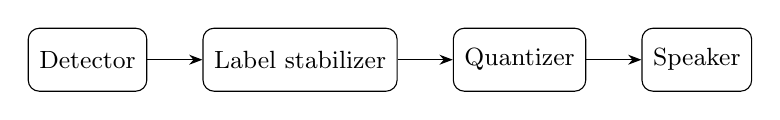
\begin{tikzpicture}[node distance=7mm, box/.style={draw, rounded corners, minimum height=8mm, inner sep=4pt, font=\small}, >=Stealth]
  \node[box] (d) {Detector};
  \node[box, right=of d] (s) {Label stabilizer};
  \node[box, right=of s] (q) {Quantizer};
  \node[box, right=of q] (t) {Speaker};
  \draw[->] (d)--(s); \draw[->] (s)--(q); \draw[->] (q)--(t);
\end{tikzpicture}
\end{center}

The \emph{description} step groups detections by (label, zone) and renders phrases such as ``very close: a person ahead''. Two quantizers are involved:
\begin{itemize}[nosep]
  \item \textbf{Position:} $c = (x_1+x_2)/(2W)$; zone is \emph{left} if $c<1/3$, \emph{right} if $c>2/3$, else \emph{ahead}.
  \item \textbf{Proximity:} $\rho = \text{box area}/\text{frame area}$; \emph{close} if $\rho\ge 0.25$, \emph{near} if $\rho\ge 0.08$, else \emph{far}.
\end{itemize}
The stabilizer keeps a label if it appears in at least $k=3$ of the last $W=5$ frames. Output is further limited by a 3\,s speech cooldown and a 15\,s repeat interval. A separate web path analyses each frame independently and therefore has no stabilizer at all.

\section{A model of boundary chatter}\label{sec:model}
Consider a static object whose true box centre (as a fraction of frame width) is $c_0$, at signed distance $d = c_0 - \tau$ from a zone threshold $\tau$. The detector reports $c_t = c_0 + \varepsilon_t$ with $\varepsilon_t \sim \mathcal{N}(0,\sigma^2)$ independent across frames (a simplification; real jitter is temporally correlated, see Section~\ref{sec:limits}). The zone on the far side of $\tau$ is reported with probability
\begin{equation}
  p(d) = \Pr(c_t < \tau) = \Phi\!\left(-\frac{d}{\sigma}\right) \quad (d>0).
\end{equation}
With independent frames, the sentence changes between consecutive frames with probability
\begin{equation}
  r(d) = 2\,p(d)\,\bigl(1-p(d)\bigr),
\end{equation}
which is maximal ($r=\tfrac12$) at $d=0$ and falls off as a Gaussian tail. Table~\ref{tab:chatter} gives values at an assumed 10 frames per second.

\begin{table}[h]
\centering
\caption{Analytic change rate for one object at distance $d$ from a threshold (independent Gaussian jitter, 10\,fps, before any speech throttling).}
\label{tab:chatter}
\begin{tabular}{rrrr}
\toprule
$d/\sigma$ & $p(d)$ & $r(d)$ per frame & changes / min \\
\midrule
0   & 0.5000 & 0.500 & 300 \\
0.5 & 0.3085 & 0.427 & 256 \\
1   & 0.1587 & 0.267 & 160 \\
2   & 0.0228 & 0.045 & 27 \\
3   & 0.0013 & 0.003 & 1.6 \\
\bottomrule
\end{tabular}
\end{table}

\paragraph{Implication.} Chatter is not a rare corner case. A person standing roughly in front of the camera has $c_0\approx 0.5$, which is far from both thresholds, but a chair at the edge of the field of view, or a person walking across the thirds boundary, spends many seconds with $d/\sigma<2$. Because the narrator speaks at most once per cooldown interval, chatter does not produce a stream of speech; instead it makes the \emph{content} of each utterance arbitrary (``on the left'' versus ``ahead'') whenever the cooldown expires.

\section{Why a label stabilizer does not help}\label{sec:stabilizer}
A $(W,k)$ stabilizer reports label $\ell$ iff it is detected in at least $k$ of the last $W$ frames. If $\ell$ is detected independently with per-frame probability $q$, the label is reported with probability $\sum_{j\ge k}\binom{W}{j}q^{j}(1-q)^{W-j}$. For $(W,k)=(5,3)$ this is $0.991$ at $q=0.9$, $0.500$ at $q=0.5$ and $0.0086$ at $q=0.1$, so it suppresses sporadic false positives well.

However, the stabilizer's key is the label only. Once $\ell$ is reported, the zone and proximity are computed from the \emph{current} frame's box, so $p(d)$ above is unchanged. A stabilizer that filters \emph{who} is described cannot make \emph{how} they are described consistent. Stabilizing per (label, zone) would be worse: an object at the threshold would alternately create and delete two groups, inflating latency for each.

\section{Hysteresis on the quantizers}\label{sec:hyst}
We propose the standard remedy used for noisy thresholds in other fields (e.g.\ the two-threshold rule in Canny edge hysteresis \cite{canny1986}): keep the previously reported zone for a tracked object unless its centre moves beyond the threshold by a margin $m$.

\begin{enumerate}[nosep]
  \item Associate each detection with the nearest previous detection of the same label (centre within a gate).
  \item If the zone computed from the current centre differs from the previous zone and $|c-\tau|<m$, keep the previous zone.
  \item Otherwise adopt the new zone.
\end{enumerate}
For an object whose true centre lies on the threshold ($d=0$) with independent Gaussian jitter, the reported zone switches in either direction with probability $\Phi(-m/\sigma)$ per frame, regardless of current state. With $m=2\sigma$ this is $0.0228$ per frame (about 14 switches/min at 10\,fps) versus 300/min without hysteresis; with $m=3\sigma$ it is $0.0013$ (about 0.8/min). The cost is a lag: a genuine crossing is reported only after the centre passes $\tau+m$, i.e.\ a spatial delay of $m$ (about $0.03$--$0.06$ of frame width for realistic $\sigma$), which at walking speeds is a fraction of a second.

The same rule applies to proximity thresholds on the area ratio $\rho$, where jitter is multiplicative; the margin should then be set on $\log\rho$.

\section{Evaluation protocol}\label{sec:protocol}
We have not run a user study. The protocol we propose is:
\begin{enumerate}[nosep]
  \item \textbf{Stimuli:} recorded indoor clips with ground-truth object positions, including objects held stationary near $c=1/3$ and $c=2/3$, and objects crossing the thresholds at walking speed.
  \item \textbf{Conditions:} (A) no filtering, (B) label stabilizer only, (C) stabilizer plus hysteresis with $m\in\{0.03,0.06\}$.
  \item \textbf{Objective metrics:} sentence-change rate per minute on static scenes; mean delay to report a true crossing; fraction of time the spoken zone matches ground truth.
  \item \textbf{Subjective metrics (blind and low-vision participants, within-subjects):} perceived reliability, mental effort (e.g.\ NASA-TLX), and the number of ``did something change?'' queries.
\end{enumerate}
The main hypothesis is that (C) lowers static-scene change rate by more than an order of magnitude without a perceptible increase in crossing delay.

\section{Limitations}\label{sec:limits}
\begin{itemize}[nosep]
  \item Frame-to-frame jitter in real detectors is temporally correlated; independent-noise results (Table~\ref{tab:chatter}) overestimate the switch rate but preserve its shape.
  \item $\sigma$ depends on detector, object size and motion blur and must be measured, not assumed.
  \item Hysteresis requires association between frames; mistaken association can freeze a wrong zone.
  \item This paper contains no empirical validation. All numbers above are analytic consequences of the stated assumptions.
\end{itemize}

\section{Related work and novelty note}
Object detection \cite{redmon2016} and the YOLOv8 implementation \cite{jocher2023} supply the raw boxes. Temporal smoothing and tracking are standard in detection pipelines, but we are not aware of prior work that treats the \emph{discretization of spatial language} in assistive narration as a stability problem. This is a claim about our own limited search and should be checked against a full literature review before submission.

\section{Conclusion}
Quantizing continuous detections into words introduces an instability at every threshold. It is invisible in per-frame accuracy metrics and untouched by label-level filtering, yet it directly affects what a listener hears. A simple two-threshold rule addresses it with a small, analyzable latency cost. The next step is to measure $\sigma$ on real footage and run the proposed study.

\begin{thebibliography}{9}
\bibitem{redmon2016} J.~Redmon, S.~Divvala, R.~Girshick, A.~Farhadi. You Only Look Once: Unified, Real-Time Object Detection. \emph{CVPR}, 2016.
\bibitem{jocher2023} G.~Jocher, A.~Chaurasia, J.~Qiu. Ultralytics YOLOv8 (software), 2023. \url{https://github.com/ultralytics/ultralytics}
\bibitem{canny1986} J.~Canny. A Computational Approach to Edge Detection. \emph{IEEE TPAMI}, 8(6):679--698, 1986.
\end{thebibliography}

\end{document}
